\documentclass[a4paper]{article}
\usepackage[italian]{babel}
\usepackage[T1]{fontenc}
\usepackage[utf8]{inputenc}
\usepackage{graphicx}
\usepackage[margin=1in]{geometry}
\usepackage{makecell}
%\usepackage[svgnames,table]{xcolor}
\usepackage[table]{xcolor}
% --- Per lo sfondo
%\usepackage{eso-pic,graphicx}
% ---
\usepackage{setspace}

\usepackage{tabularx} 

\usepackage[hidelinks]{hyperref}
\usepackage{array}

\usepackage{fancyhdr}
\usepackage{float}

% Definizione comandi personali - Team
\newcommand{\FP}{Francesco Protopapa}
\newcommand{\GC}{Greta Cavedon}
\newcommand{\LW}{Luciano Wu}
\newcommand{\PV}{Pietro Villatora}
\newcommand{\EP}{Edoardo Pavan}
\newcommand{\MG}{Michele Gatto}
\newcommand{\MB}{Matteo Basso}

% Definizione File
\newcommand{\G}{\textit{Glossario v1.0.0}}
\newcommand{\AdR}{\textit{Analisi dei Requisiti v1.0.0}}
\newcommand{\PdP}{\textit{Piano di Progetto v1.0.0}}
\newcommand{\PdQ}{\textit{Piano di Qualifica v1.0.0}}
\newcommand{\SdF}{\textit{Studio di fattibilità v1.0.0}}
\newcommand{\NdP}{\textit{Norme di Progetto v1.0.0}}

% Definizione ruoli
\newcommand{\AN}{Analista}
\newcommand{\VE}{Verificatore}
\newcommand{\AM}{Amministratore}
\newcommand{\RE}{Responsabile}
\newcommand{\PT}{Progettista}
\newcommand{\PR}{Programmatore}

\newcommand{\glo}{\textsuperscript{G}}

%Abbreviaizoni requisiti
\newcommand{\Ob}{Obbligatorio}
\newcommand{\De}{Desiderabile}
\newcommand{\Fa}{Facoltativo}

%Abbrevizioni fonti requisiti
\newcommand{\Di}{Decisione interna}
\newcommand{\Vi}{Verbale interno}
\newcommand{\Ve}{Verbale esterno}
\newcommand{\Ca}{Capitolato}

%link in blu
\newcommand{\mylink}[1]{\color{blue}\url{#1}\color{black}}
\makeindex

\usepackage{longtable}

% Per evidenziare il testo
\usepackage{tcolorbox}



\setcounter{secnumdepth}{4}
\setcounter{tocdepth}{4}

\begin{document}

	% Intro documento 

\begin{center}

\begin{figure}
\centering

\includegraphics[scale=0.05]{Contenuto/Immagini/DreamTeam.png} 
\end{figure}

{\Huge{\textbf{Norme di Progetto}}} \\ [1cm]

\begin{table}[htbp]
\centering
\begin{tabular}{r|c}
\multicolumn{2}{c}{\textbf{Informazioni sul Documento}} \\
\hline \\
\textbf{Versione} & 3.0.0 \\ \rule{0pt}{3ex}    
\textbf{Data di approvazione} & 2022-06-18  \\ \rule{0pt}{2ex} 
\textbf{Approvatori} & \MB{} \\ \rule{0pt}{3ex}      
\textbf{Redattori} & \MG{} \\ \rule{0pt}{2ex}   
& \PV{} \\ \rule{0pt}{3ex}    
\textbf{Verificatori} 
  & \GC{} \\ \rule{0pt}{2ex}
& \EP{} \\ \rule{0pt}{2ex} 
      
\textbf{Uso} & Interno \\ \rule{0pt}{3ex}    
\textbf{Distribuzione} & Prof. Vardanega Tullio \\ \rule{0pt}{2ex}   
& Prof. Cardin Riccardo \\ \rule{0pt}{2ex}   
& Gruppo \textit{DreamTeam} \\ \rule{0pt}{0.1cm}   
\end{tabular} \\ [0.5cm]
\end{table}

\textsl{ e-mail: \href{mailto:dreamteam.unipd@gmail.com}{dreamteam.unipd@gmail.com} } \\[2cm]
\end{center}
\pagebreak	
	% Inserimento di header e footer

\pagestyle{fancy}
\fancyhf{}
\rhead{Piano di Progetto}
\lhead{
\includegraphics[scale=0.015]{Sezioni/images/DreamTeam.png}}
\rfoot{\thepage}
\setlength{\headheight}{35pt}


%\cfoot{Pagina \thepage}
%\setlength{\headheight}{35pt}
%\setcounter{tocdepth}{5}
%\setcounter{secnumdepth}{5}
%\renewcommand{\footrulewidth}{0.4pt}
	% Registro Modifiche

\definecolor{darkblue}{cmyk}{99, 99, 0, 71}

{\LARGE{\textbf{Registro delle Modifiche}}} \\
\begin{table}[!htbp]
\rowcolors{2}{gray!25}{white}
\renewcommand{\arraystretch}{1.5}
\begin{tabular}{ m{0.1\textwidth}<{\centering}  m{0.11\textwidth}<{\centering}  m{0.2\textwidth}<{\centering}  m{0.17\textwidth}<{\centering}  m{0.3\textwidth}<{\centering} }
	\rowcolor{darkblue}
	\textcolor{white}{\textbf{Versione}} &\textcolor{white}{\textbf{Data}}& \textcolor{white}{\textbf{Nominativo}} & \textcolor{white}{\textbf{Ruolo}}&\textcolor{white}{\textbf{Descrizione}}\\ 
	v1.0.0& 2022-01- & \shortstack{ \\ XX} &\shortstack{ \\ \RE{} } & Approvazione del documento \\

	v0.0.1& 2022-01-14 & \shortstack{ \\ \GC{}} &\shortstack{ \\ \AN{} } & Realizzazione struttura in Latex e stesura documento; \VE: \textit{}\\

\end{tabular}
\end{table}

\pagebreak	
		
	% indice
	\renewcommand{\contentsname}{Indice}
	\tableofcontents	
	\listoffigures
	%\listoftables
	\pagebreak
	
	% contenuto del documento, ogni sezione in un file
	\section{Introduzione}

\subsection{Scopo del Documento}
Lo scopo del presente documento è quello di descrivere in maniera coesa, coerente ed esaustiva le caratteristiche architetturali del prodotto \textit{Sweeat} sviluppato dal gruppo \textit{DreamTeam}.


\subsection{Scopo del Prodotto}
L’obiettivo di Sweeat e dell’azienda \zd è la creazione di un sistema software costituito da una Webapp. Lo scopo del prodotto è di fornire all’utente una guida dei locali gastronomici sfruttando i numerosi contenuti digitali creati dagli utenti sulle principali piattaforme social (Instagram e TikTok).
In questo modo, è possibile realizzare una classifica basata sulle impressioni e reazioni di chiunque usufruisca dei servizi dei locali, non solo da professionisti ed esperti del settore.


\subsection{Glossario}
Per evitare ambiguità relative alle terminologie utilizzate è stato creato un documento denominato “\textit{Glossario}”. Questo documento comprende tutti i termini tecnici scelti dai membri del gruppo e utilizzati nei vari documenti con le relative definizioni. Tutti i termini inclusi in questo glossario, vengono segnalati all'interno del documento con l'apice \textsuperscript{G} accanto alla parola.

\subsection{Riferimenti}
\subsubsection{Normativi}
\begin{itemize}
\item \textit{Analisi dei Requisiti v2.0.0}
\item Presentazione del capitolato - Zero12 Progettazione e sviluppo di una Social guida Michelin:
\newline \mylink{https://www.math.unipd.it/~tullio/IS-1/2021/Progetto/C4p.pdf}
\end{itemize}
\subsubsection{Informativi}
\begin{itemize}
\item Regolamento del progetto didattico - Materiale didattico del corso di Ingegneria del Software:
\newline \mylink{https://www.math.unipd.it/~tullio/IS-1/2021/Dispense/PD2.pdf}
\begin{itemize}
\item \textit{Slides 12, 17.}
\end{itemize}
\item Diagrammi delle classi - Materiale didattico del corso di Ingegneria del Software:
\newline \mylink{https://www.math.unipd.it/\%7Ercardin/swea/2021/Diagrammi\%20delle\%20Classi_4x4.pdf}
\item Design Pattern Strutturali - Materiale didattico del corso di Ingegneria del Software:
\newline \mylink{https://www.math.unipd.it/\%7Ercardin/swea/2021/Design\%20Pattern\%20Strutturali_4x4.pdf}
\begin{itemize}
\item \textit{Slides 4-13, 25-34.}
\end{itemize}
\item Design Pattern Comportamentali - Materiale didattico del corso di Ingegneria del Software:
\newline \mylink{https://www.math.unipd.it/\%7Ercardin/swea/2021/Design\%20Pattern\%20Comportamentali_4x4.pdf}
\begin{itemize}
\item \textit{Slides 32-40.}
\end{itemize}
\item Model-View Patterns - Materiale didattico del corso di Ingegneria del Software:
\newline \mylink{https://www.math.unipd.it/~rcardin/sweb/2022/L02.pdf}
\begin{itemize}
\item \textit{Slides 31-40.}
\end{itemize}
\item Static Factory - Cleaner Code with Static Factory Methods:
\newline \mylink{https://stackify.com/static-factory-methods/}
\end{itemize} 
	\pagebreak
	\section{Architettura del Prodotto}

\subsection{Architettura generale}

\subsubsection{Schema}
\begin{figure}[H]
    \centerfloat
    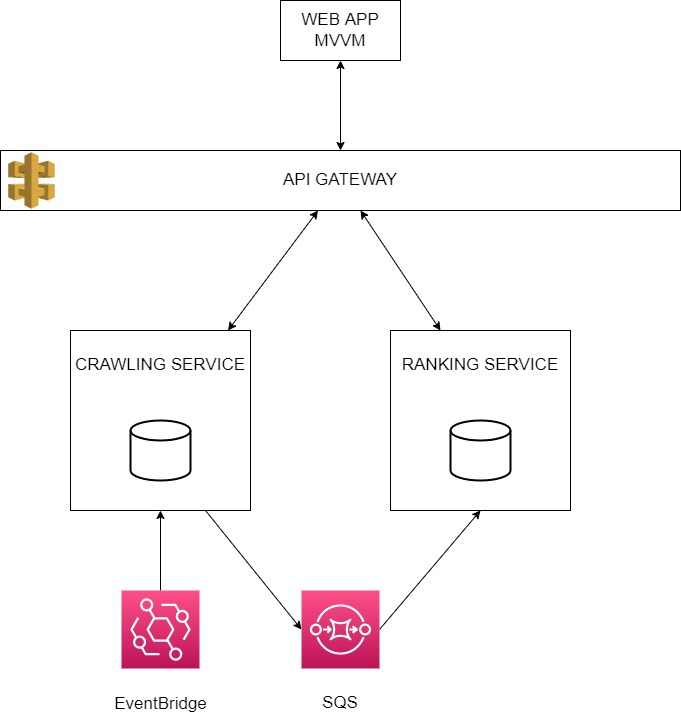
\includegraphics[scale=0.35]{Contenuto/Immagini/backend-architettura.jpg}
    \caption{Architettura generale}
\end{figure}

\subsubsection{Descrizione}
Come richiesto dal capitolato si è deciso di utilizzare un'architettura a microservizi, i quali comunicano con il Frontend tramite API Gateway\glo.
In particolare sono stati individuati i seguenti microservizi:
\begin{itemize}
    \item \textit{Crawling Service}: questo microservizio si occupa di tutto ciò che riguarda il crawling dei dati da Instagram. Il processo di crawling viene innescato da un servizio di AWS chiamato EventBridge\glo che si occupa dello scheduling del crawling. Ogni volte che viene trovato dal crawler un post relativo ad un ristorante, questo viene inviato ad una coda SQS\glo dalla quale andrà a leggere il servizio di ranking. Infine il Crawling Service espone una API al Frontend per permettere di suggerire profili Instagram da aggiungere alla lista di quelli osservati dal crawler.
    \item \textit{Ranking Service}: questo microservizio invece si occupa dell'analisi dei contenuti estratti dal crawler e della realizzazione di una classifica di ristoranti. Il processo di analisi di un post viene fatto partire dalla ricezione di un messaggio sulla coda SQS, una volta letto il messaggio esso viene rimosso dalla coda ed analizzato. Infine il Ranking Service espone molteplici API al Frontend in grado di fornire tutte le informazioni necessarie per poter visualizzare la classifica, i dettagli di un locale e la gestione dei preferiti.
\end{itemize}

Invece, per il Frontend è stato scelto di realizzare la struttura sfruttando il pattern architetturale \textit{Model-View-ViewModel} (MVVM), il quale comunica con il Backend esclusivamente tramite API Gateway.

Possiamo riassumere le motivazioni per cui abbiamo scelto il pattern architetturale MVVM per la parte Frontend come segue:

\begin{itemize}
\item La parte di Front-end è stata realizzata sfruttando la libreria React\glo che si integra particolarmente bene con il pattern MVVM,
\item Permette di riutilizzare i vari componenti in diversi contesti senza dover effettuare modifiche; un esempio è il modello che sfruttiamo per estrarre dati dal database, i quali (tramite la stessa chiamata) vengono usati in diverse pagine della WebApp. Lo stesso vale per la vista (perché usiamo un componente in diverse pagine della WebApp),
\item Permette di disaccoppiare la parte di business logic dalla presentation logic, aspetto che rende più semplice anche i test di unità,
\item Maggior semplicità di sviluppo in team: in questo modo, ogni singolo componente del gruppo può occuparsi di una sola parte della WebApp,
\item Manutenibilità più semplice, per via del disaccoppiamento del codice.
\end{itemize}
Inoltre, per la parte di autenticazione è stato utilizzato Cognito\glo, un servizio di AWS consigliatoci dall'azienda \textit{Zero12}, che permette di creare e gestire bacini d'utenza, oltre al framework AWS Amplify\glo per la parte di hosting ed autenticazione lato Frontend.

\subsubsection{Comunicazione tra servizi}
Per implementare la comunicazione tra il Crawling Service e Ranking Service viene utilizzata una coda SQS. La scelta di utilizzare il servizio SQS deriva da due motivi principali:
\begin{itemize}
\item Il servizio è completamente gestito da AWS, con un uptime del 99 \% ;
\item Si integra nativamente con il servizio Lambda\glo ;
\item Costi ridotti
\end{itemize}

\paragraph{Impostazioni coda SQS}
\'E stata scelta una coda di tipo \textbf{FIFO} poiché garantisce l'elaborazione unica di ogni messaggio e gestisce internamente i duplicati, cancellandoli. Questo viene a costo delle performance, che non sono una criticità poiché il servizio di analisi di Ranking Service lavora in background, consumando i messaggi ad una velocità ridotta.
Di seguito alcuni parametri impostati:
\begin{itemize}
\item \textbf{Visibility Timeout}: il tempo che un messaggio rimane nascosto dopo essere ricevuto da un consumatore. Impostato a 20 minuti poiché deve essere maggiore del tempo di esecuzione della Lambda che effettua l'analisi, che è di 15 minuti;
\item \textbf{Message retention period}: il tempo massimo di permanenza dei messaggi nella coda. Impostato a 2 giorni;
\item \textbf{Maximum message size}: La dimensione massima del messaggio. Impostata a 256 KB, che è la massima dimensione e quella consigliata da AWS.
\item \textbf{Receive message wait time}: Il tempo massimo che il consumatore aspetta per i messaggi che diventino disponibili. Impostata a 20 secondi, che è il tempo massimo. Questo riduce il consumo di risorse, perché ora aspetta 20 secondi prima di ritornare una risposta vuota e permette al consumatore di lavorare sempre a pieno regime, in quanto aspettando 20 secondi la coda fa in tempo a riempirsi di almeno un batch completo;
\item \textbf{Dimensione batch}: Il massimo numero di messaggi che un consumatore riceve per volta. Impostato a 10 che è il massimo per le code FIFO. In questo modo vengono ridotte le chiamate al servizio di analisi.
\end{itemize}

\paragraph{Dead letter queue}
Una dead letter queue (DLQ) è una coda agguntiva utilizzata per gestire i messaggi che non vengono elaborati con successo.
Il suo utilizzo si è ritenuto necessario per spostare della codapricipale  i messaggi che generavano errori, permettendo a quelli corretti di essere elaborati, e quindi sbloccando la coda. Quindi i messaggi non corretti vengono spostati nella DLQ e possono essere analizzati in sede separata. I motivi principali per cui è stato scelto di usare una DLQ sono la semplificazione del testing e debug, permettendo di mantenere il servizio in funzione e la possibilità di reindirizzare nella coda principale i messaggi che generavano errore (dopo che il problema è stato individuato e risolto) evitando di perderli.
Di seguito alcuni dei parametri impostati:
\begin{itemize}
\item \textbf{Message retention period}: Impostato al suo valore massimo, 14 giorni, così da far pemanere più tempo possibile i messaggi che generano errore;
\item \textbf{Maximum Receives}:  Il numero massimo di volte che il messaggio viene ricevuto ed elaborato senza successo. Impostato a 3, quindi dopo la seconda elaborazione senza successo viene messo nella DLQ. Il valore è stato deciso empiricamente, in questo modo i messaggi vengono ritentati per 3 volte nel giro di un'ora (20 minuti di visibility timeout). L'idea è che in generale un eventuale problema di downtime di qualche servizio possa essere mitigato e al tempo stesso si evita di riprovare troppe volte un messaggio che genera errore nel codice delle procedure, poiché finché non viene corretto, verrà continuamente generato lo stesso errore, sprecando risorse ed impedendo ad eventuali altri messaggi corretti di venire elaborati. 
\end{itemize}
In generale il resto delle impostazioni resta identico a quello della coda principale.


\pagebreak

\subsection{Architettura del Crawling Service}

\subsubsection{Descrizione}
Il microservizio denominato \textit{Crawling Service} si occupa principalmente di due funzionalità:
\begin{itemize}
    \item Crawling dei dati: questo processo avviene tramite l'utilizzo della libreria Instagrapi. Ogni volta che viene chiamato il metodo start\_crawling della classe FacadeCrawling, il sistema sceglie dal proprio database il profilo instagram che non viene guardato da più tempo e ne effettua il crawling dei dati. Per ogni media prelevato dal profilo, viene analizzata la sua location e nel caso in cui essa sia quella di un ristorante, il media viene salvato nel database ed inviato alla coda SQS in modo che possa essere analizzato dal servizio \textit{Ranking Service};
    \item Suggerimento dei profili: questa funzionalità viene esposta tramite una API rest al frontend al fine di fornire all'utente la possibilità di suggerire un profilo instagram sul quale successivamente il sistema andrà ad effettuare il crawling dei dati. Prima di essere aggiunto al database, viene controllato che il profilo non sia già presente, esista e sia pubblico. In base a ciascun esito verrà restituito il corrispettivo ritorno.
\end{itemize}

\subsubsection{Diagrammi delle classi}
\begin{figure}[h]
    \centering
    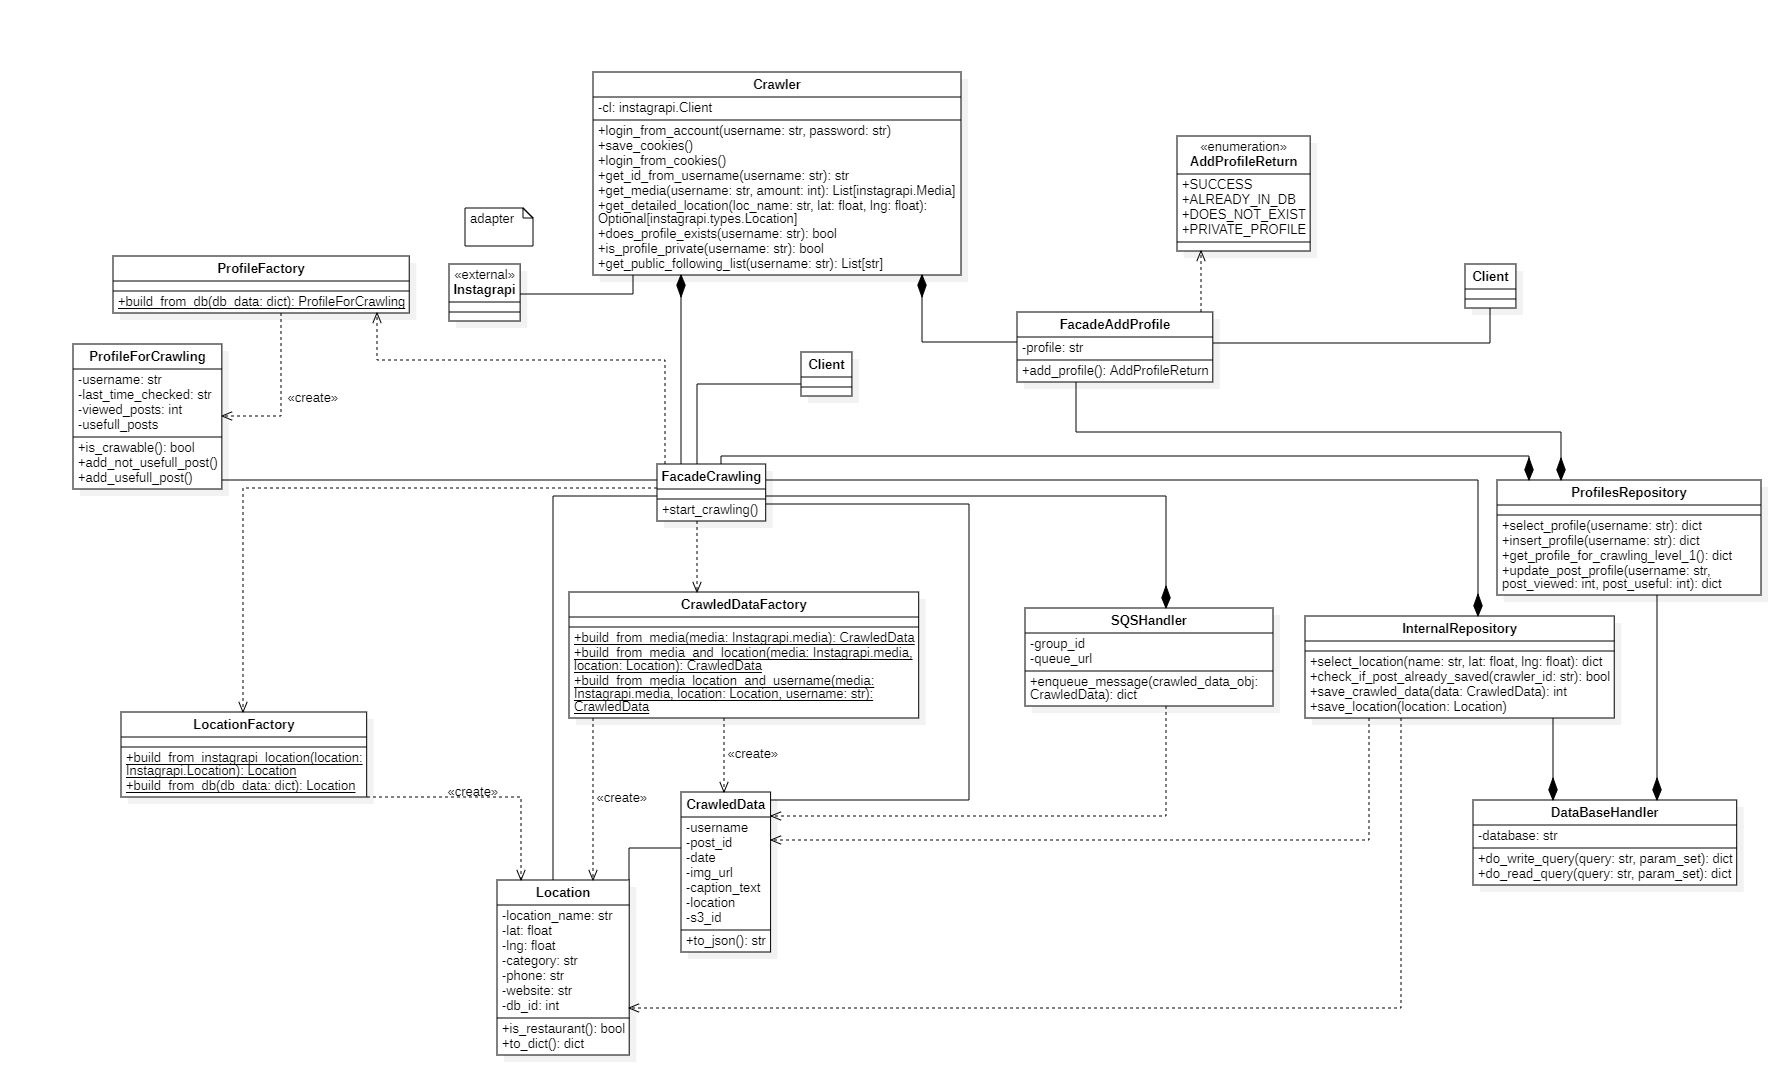
\includegraphics[scale=0.35]{Contenuto/Immagini/classi-CS.JPG}
    \caption{Crawling Service - Diagramma delle classi}
\end{figure}
\subsubsection{Diagrammi di sequenza}
In questa sezione vengono presentati i diagrammi di sequenza che modellano le operazioni principali del Crawling Service:
\begin{itemize}
    \item il suggerimento di un profilo instagram da aggiungere alla lista dei profili su cui viene effettuato il crawling dei dati, nel caso in cui il profilo non sia già presente e sia pubblico;
    \item il processo di crawling dei dati;
    \item la formattazione di un singolo media ottenuto tramite crawling
\end{itemize}
\begin{figure}[!htp]
    \centering
    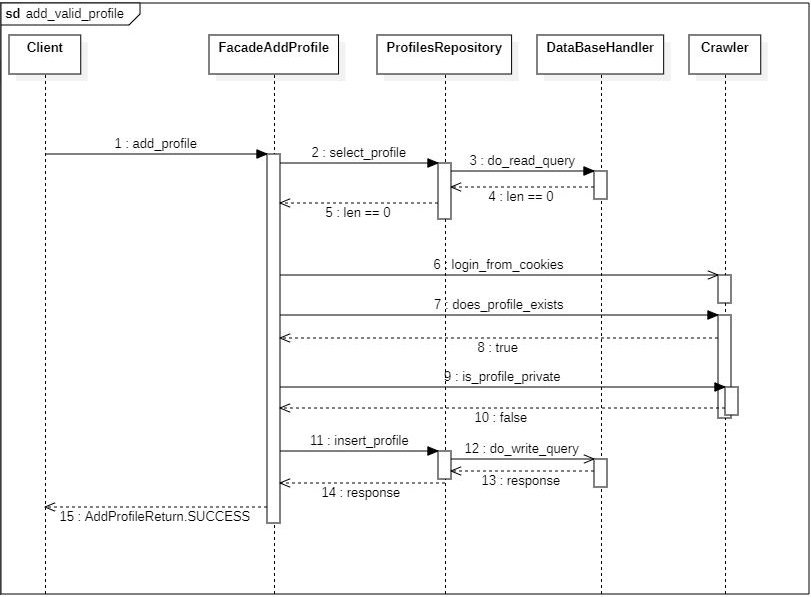
\includegraphics[scale=0.65]{Contenuto/Immagini/seq1-CS.JPG}
    \caption{Crawling Service - Diagramma di sequenza - 1}
\end{figure}
\begin{figure}[H]
    \centerfloat
    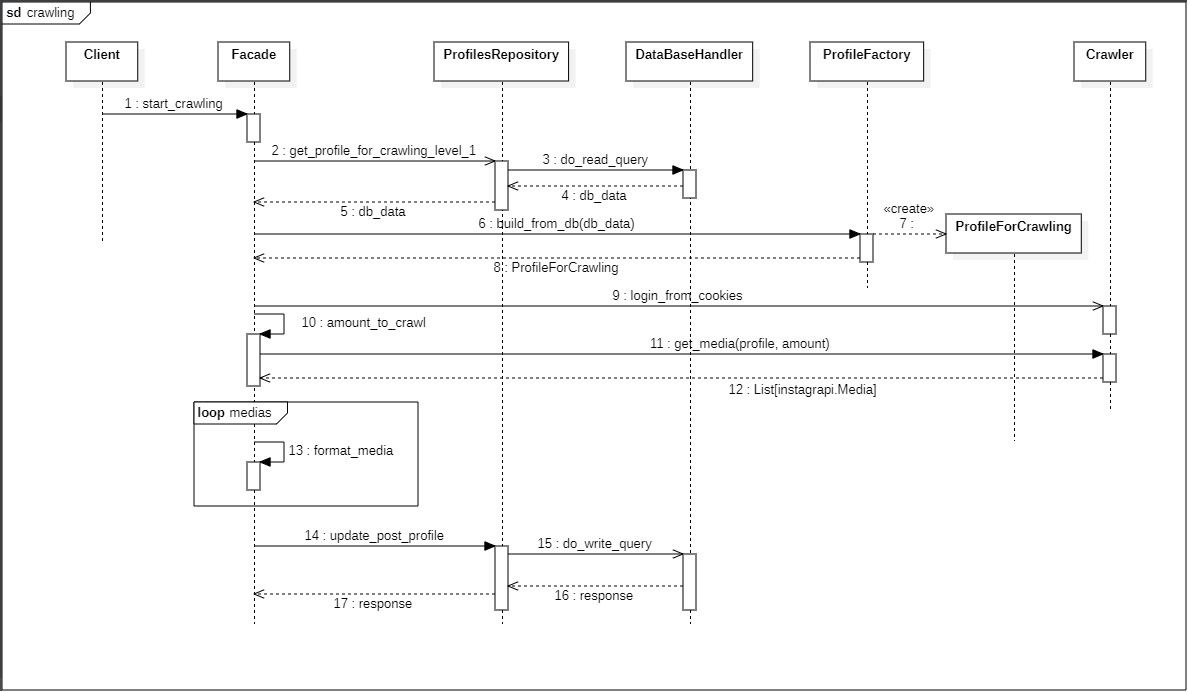
\includegraphics[scale=0.55]{Contenuto/Immagini/seq2-CS.JPG}
    \caption{Crawling Service - Diagramma di sequenza - 2}
\end{figure}
\begin{figure}[!htp]
    \centering
    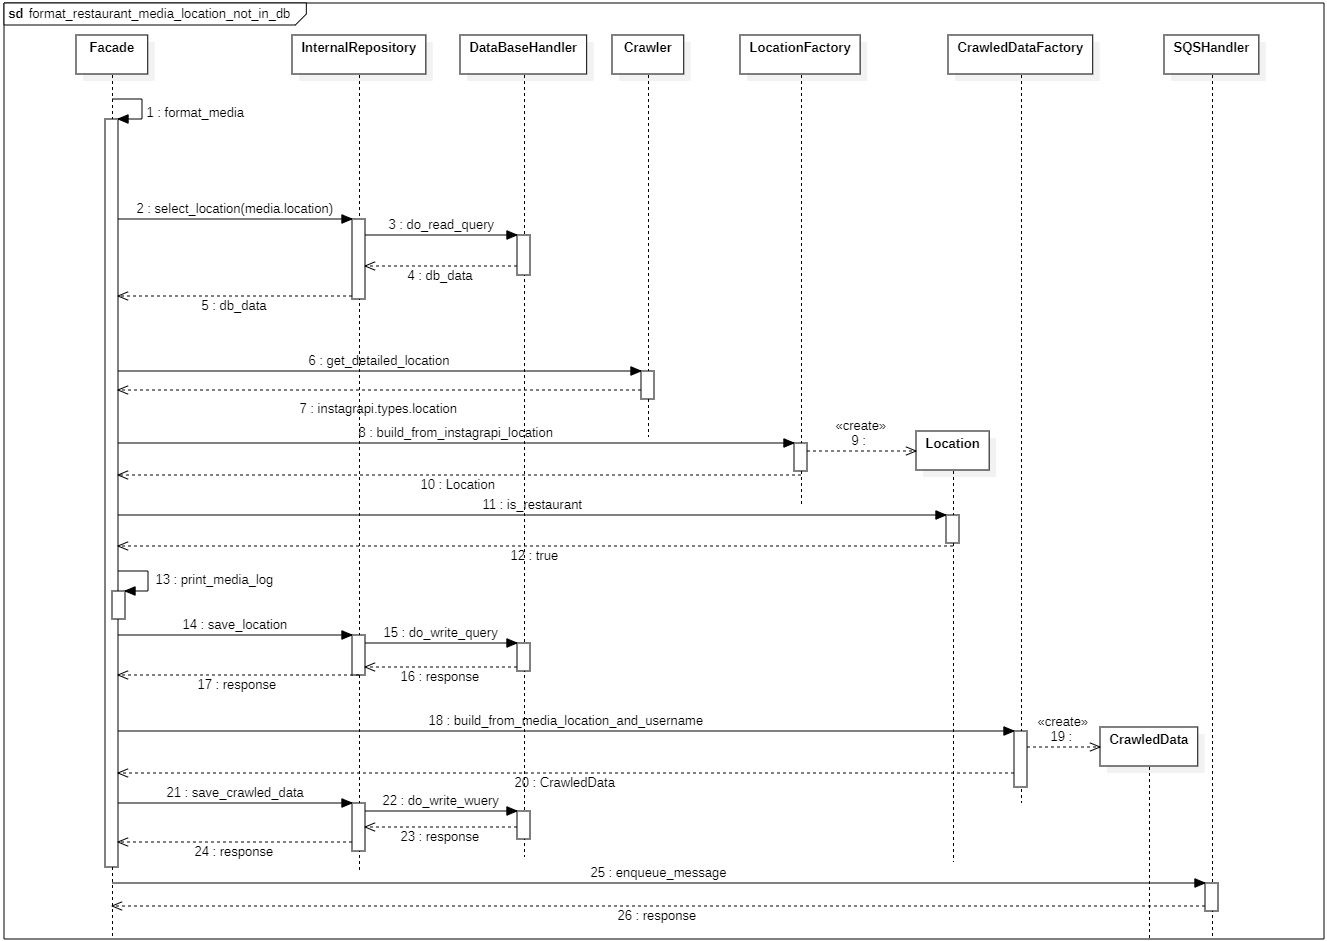
\includegraphics[scale=0.45]{Contenuto/Immagini/seq3-CS.JPG}
    \caption{Crawling Service - Diagramma di sequenza - 3}
\end{figure}

\subsection{Struttura messaggio SQS}
\begin{figure}[H]
    \centerfloat
    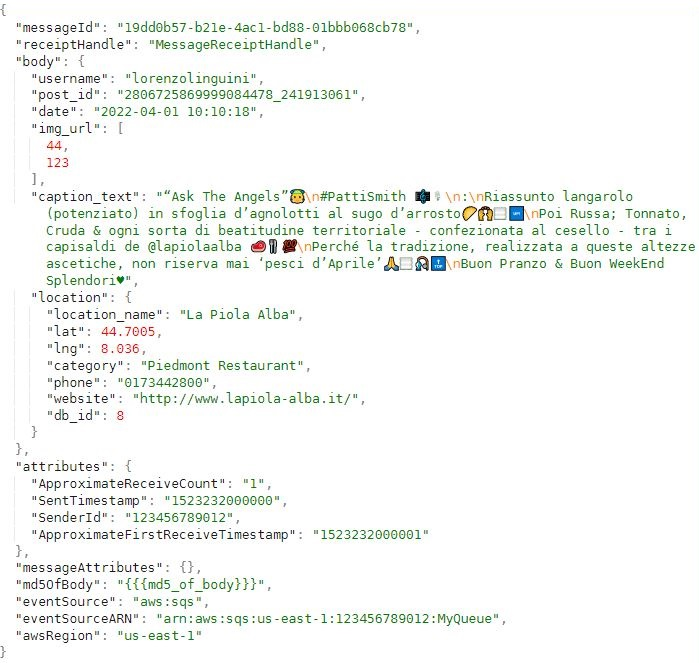
\includegraphics[scale=0.55]{Contenuto/Immagini/messaggiosqs.JPG}
    \caption{Crawling Service - Esempio di un messaggio SQS}
\end{figure}

\subsubsection{Design pattern notevoli utilizzati}
Per La realizzazione del Crawling Service sono stati utilizzati i seguenti design pattern:
\begin{itemize}
    \item \textbf{Facade:} Utilizzato per la realizzazione delle classi FacadeCrawling e FacadeAddProfile, in modo da fornire ai client un'interfaccia semplice ad un sottosistema molto complesso e disaccoppiando la logica di implementazione del sistema dal client.
    \item \textbf{Adapter:} Utilizzato dalla classe Crawler pre disaccoppiare il resto del sistema dai metodi di instagrapi, rendendo disponibili solo quelli necessari tramite un'interfaccia nota al sistema.
    \item \textbf{Static Factory:} Utilizzato per fornire dei metodi statici in grado di creare oggetti di tipo CrawledData, Location, ProfileForCrawling a partire da altri tipi di oggetti.
\end{itemize}

\subsubsection{Schema del database}
\begin{figure}[h]
    \centering
    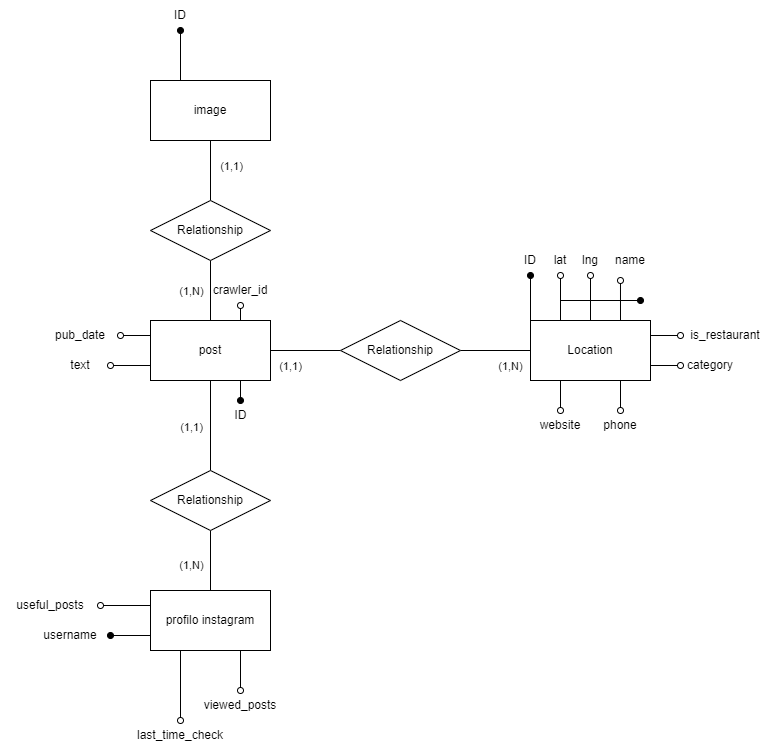
\includegraphics[scale=0.35]{Contenuto/Immagini/ER-CS.png}
    \caption{Crawling Service - Schema ER del database}
\end{figure}
\pagebreak

\subsection{Architettura del Ranking Service}
\subsubsection{Descrizione}
Il microservizio denominato \textit{Ranking Service} svolge le seguenti funzionalità:
\begin{itemize}
	\item Gestione della classifica: ogni volta che un nuovo messaggio () viene aggiunto alla coda SQS, viene chiamati il metodo \texttt{refresh\_ranking} che si occupa di recuperare e fare la parsificazione\glo e deserializzazione\glo dei messaggi nella coda (lavorando a batch di massimo 10 messaggi). Dopo di che i messaggi vengono analizzati tramite i servizi Comprehend\glo e Rekognition\glo di AWS e vengono generati i punteggi per le foto, per il testo e per le emoji. Viene quindi aggiornato il database, aggiungendo il ristorante e il media (se non presenti) e aggiornati i punteggi.
	Vengono inoltre esposti due API endpoint:
		\begin{itemize}
			\item \texttt{getRanking}: restituisce una parte della classifica generale;
			\item \texttt{getLabelAndPost}: restituisce i media (e le relative label\glo) di un particolare ristorante.
		\end{itemize}
	\item Funzionalità di ricerca: viene esposto un API endpoint \texttt{searchByName} che restituisce tutte le informazioni presenti nel database relative ad un ristorante con un nome specifico (media compresi); 
	\item Gestione dei preferiti: viene esposto un API endpoint \texttt{favorites} che abilità alla gestione della lista di ristoranti preferiti per ogni utente, fornendo le funzionalità di aggiunta, rimozione e visualizzazione per la lista dei preferiti.
\end{itemize}

\subsubsection{Diagrammi delle classi}
\begin{figure}[H]
    \centerfloat
    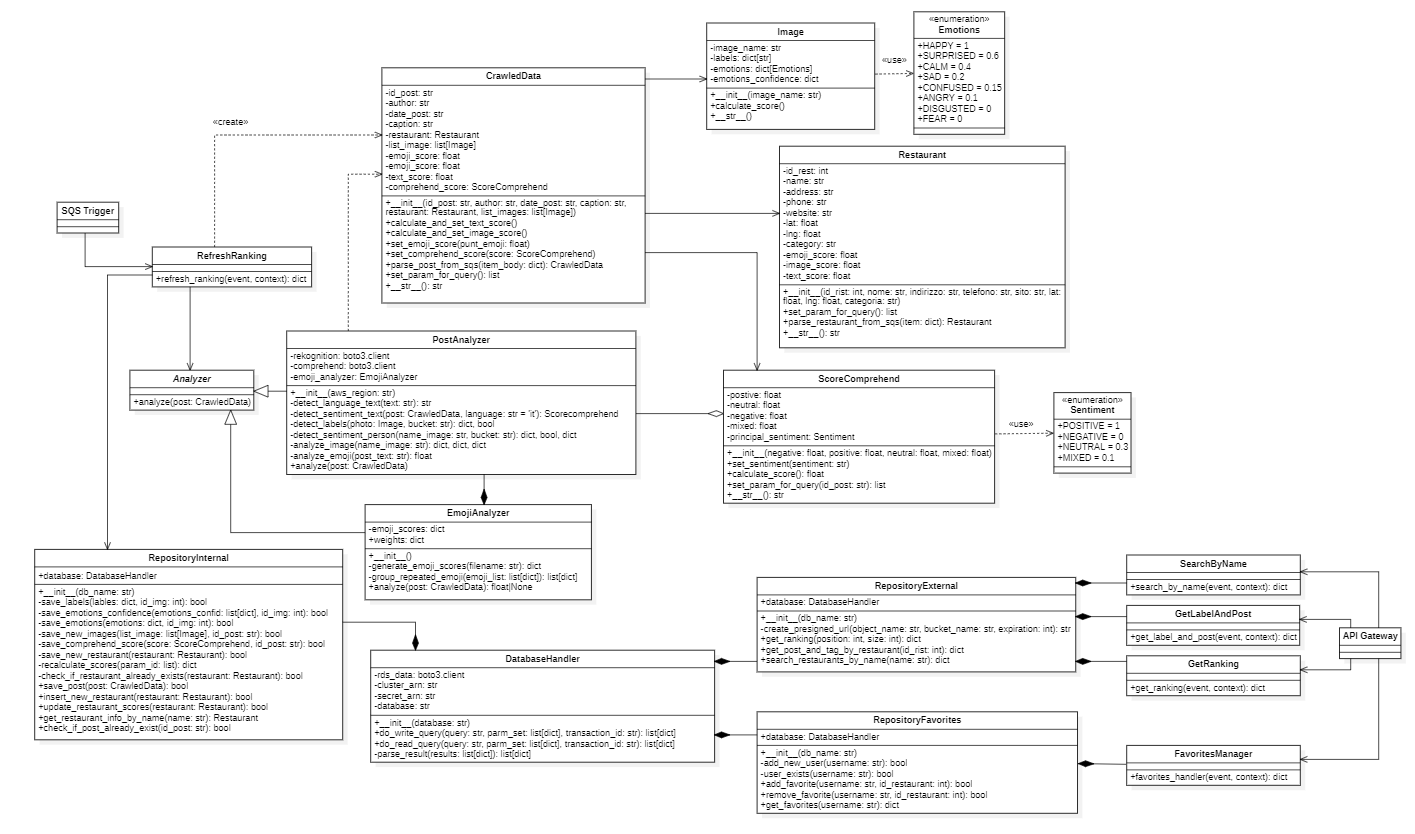
\includegraphics[scale=0.35]{Contenuto/Immagini/classi-RS.jpg}
    \caption{Ranking Service - Diagramma delle classi}
\end{figure}

\subsubsection{Diagrammi di sequenza}
In questa sezione vengono presentati i diagrammi di sequenza che modellano le operazioni principali del Ranking Service:
\begin{itemize}
	\item Il processo di analisi di un media, assumendo che il media e il ristorante non siano già presenti nel database e che siano presenti persone delle immagini;
	\item Il processo di salvataggio del media analizzato e del ristorante, sempre assumendo che il media e il ristorante non siano già presenti nel database, e l'aggiornamento dei punteggi.
\end{itemize}
\begin{figure}[H]
    \centerfloat
    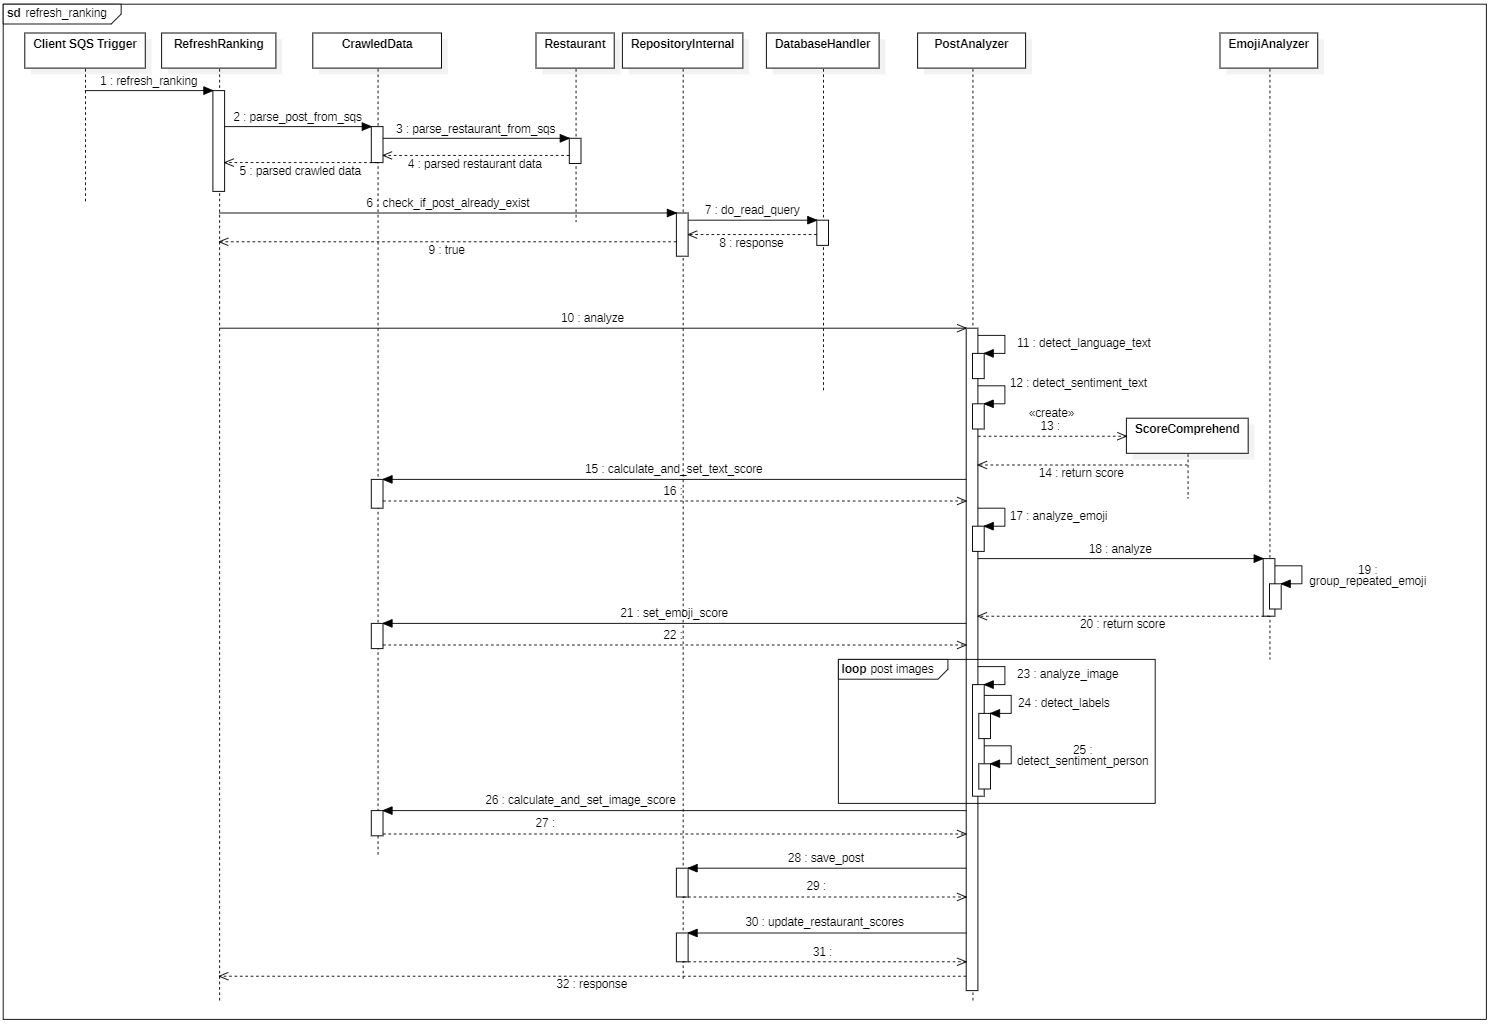
\includegraphics[scale=0.45]{Contenuto/Immagini/seq1-RS.JPG}
    \caption{Ranking Service - Diagramma di sequenza - 1}
\end{figure}
\begin{figure}[H]
    \centering
    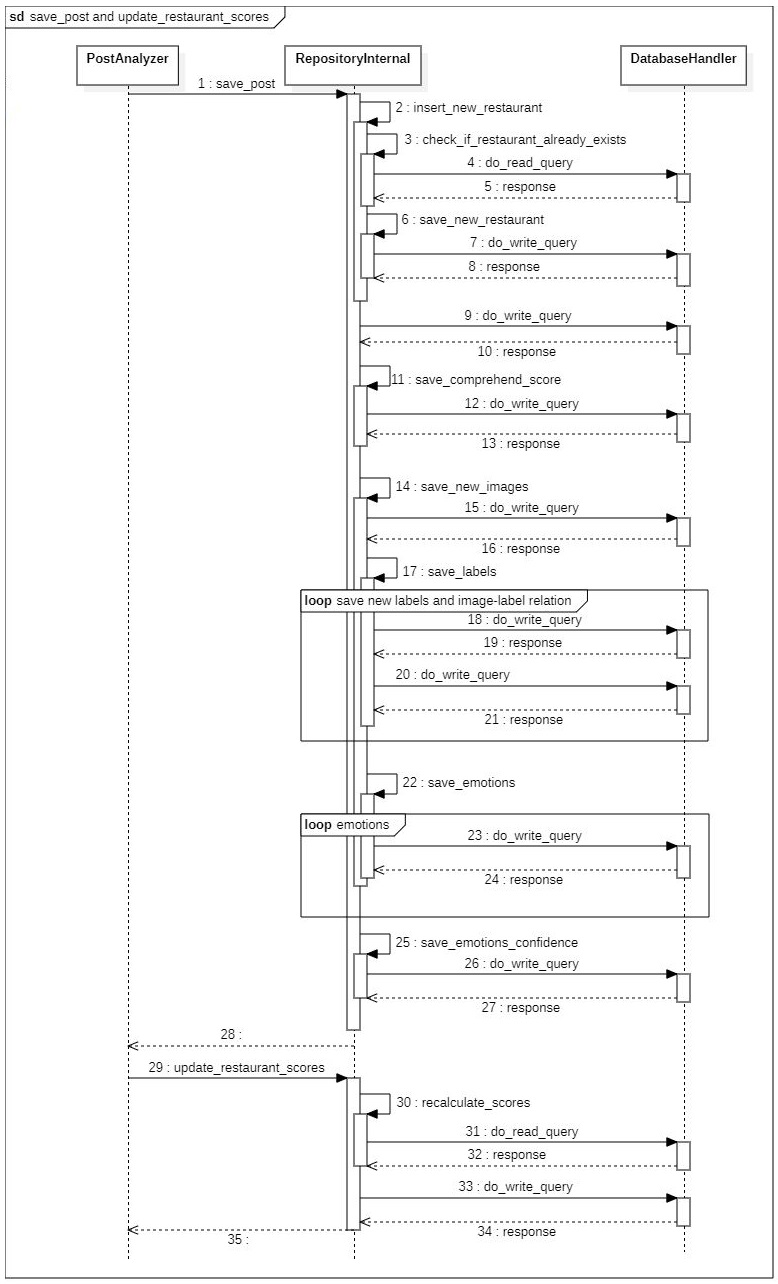
\includegraphics[scale=0.55]{Contenuto/Immagini/seq2-RS.JPG}
    \caption{Ranking Service - Diagramma di sequenza - 2}
\end{figure}

\subsubsection{Note sul processo di analisi}
Dopo alcune prove ed osservazioni sono state fatte alcune decisioni relative al processo di analisi:
\begin{itemize}
	\item Dopo l'analisi della immagini, verranno salvate nel database solo le label relative al cibo (quindi con padre "Food") e con confidenza di almeno il 90\%;
	\item Solo se nelle immagini viene trovata la label "Person" verrà effettuata l'analisi dei sentimenti nell'immagine tramite Rekognition, anche in questo caso verranno salvati solo i sentimenti predominanti con una confidenza di almeno il 90\%.
\end{itemize}

\subsubsection{Design pattern notevoli utilizzati}
Per La realizzazione del Ranking Service sono stati utilizzati i seguenti design pattern:
\begin{itemize}
    \item \textbf{Strategy:} Utlizzato per la realizzazione di PostAnalyzer ed EmojiAnalyzer, è stato scelto principalmente per la sua versatilità.\\
    Questo pattern infatti ci permette, nel caso in cui in futuro ci sia bisogno di un algoritmo più avanzato per l'analisi dei post, con il minimo sforzo e modifica del codice, di implementare la nuova classe che erediterà anch'essa dalla classe base Analyzer.
    \item \textbf{Static Factory:} Utilizzato per la creazione di oggetti dalle varie fonti accessibili dal microservizio, come la coda SQS, e la creazione di liste contenti dati pronti per l'utilizzo nei metodi riguardanti il database.
\end{itemize}

\subsubsection{Schema del database}
\begin{figure}[h]
    \centering
    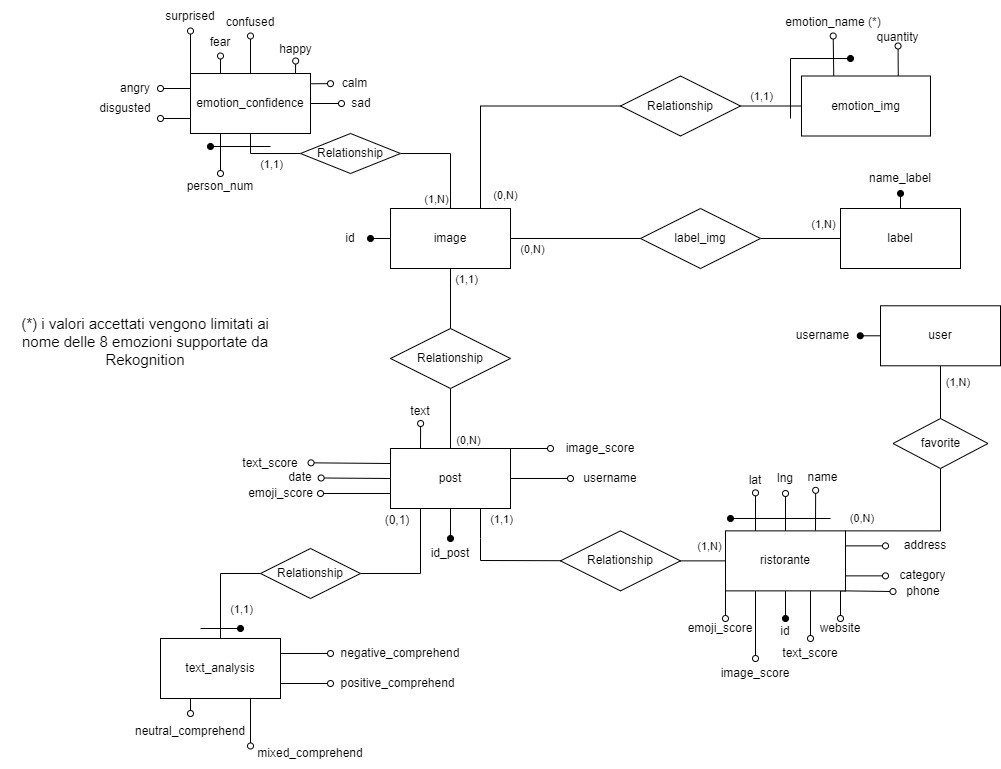
\includegraphics[scale=0.35]{Contenuto/Immagini/ER-RS.jpg}
    \caption{Ranking Service - Schema ER del database}
\end{figure}
\pagebreak

\subsection{Architettura del FrontEnd}
\pagebreak
	\pagebreak
	\section{Requisiti Soddisfatti}
	\pagebreak
	
\end{document}